\documentclass{jtetiproposalskripsi}

\titleind{SISTEM PENGORGANISASIAN DATA TAMU DENGAN DUKUNGAN JARINGAN NIRKABEL DAN ANDROID PADA EVENT ORGANIZER PERNIKAHAN}

\fullname{ASA ISA FIRMANSYAH}

\idnum{1410651073}

\degree{Sarjana Teknik Informatika}

\yearsubmit{2014}

\program{Teknik Informatika}

\dept{Teknik}


\begin{document}

\cover

\begin{abstractind}
Sampai saat ini suatu permasalahan yang ada pada acara pernikahan yaitu masih menggunakannya buku tamu sebagai bukti kehadiran para tamu. Hal ini menyebabkan tidak terorganisasinya data tamu sehingga data akan sulit direkap sesudah acara  pernikahan. Kendala lain yaitu muncul disaat penerima tamu undangan melayani tamu undangan yang hadir, karena penerima tamu undangan tidak bisa membedakan tamu-tamu khusus dan tamu biasa yang datang di acara tersebut. Hal ini mengakibatkan acara tidak terorganisasi karena pengantin dan keluarga sulit untuk mengetahui siapa saja tamu istimewa  yang datang dan mengambil objek gambar untuk dijadikan kenangan pada acara resepsi pernikahan.

Dengan berkembangnya teknologi informasi, maka perlu diciptakan suatu aplikasi untuk membantu panitia pernikahan \emph{(event organizer)} dalam menyelesaikan permasalahan tersebut. Yaitu dengan menggunakan sistem \emph{database} pada data tamu agar dapat tersusun rapi dan mudah untuk direkap atau dijadikan sebuah laporan. \emph{Barcode} dapat digunakan untuk menscan undangan tamu yang hadir dengan tujuan mengetahui data tamu yang sudah disimpan pada \emph{database} dan untuk merubah status pada \emph{database} dari status tidak hadir menjadi hadir. Ini akan mempermudah penerima tamu undangan untuk menerima tamu undangan yang hadir di acara resepsi pernikahan karena secara otomatis data tamu akan muncul pada aplikasi di komputer yang saling terhubung dengan \emph{database}. Acara pun dapat terorganisisasi dengan baik karena data yang sudah discan dan  masuk dalam \emph{database} akan ditransfer pada aplikasi android yang akan memunculkan notifikasi secara cepat dengan dukungan jaringan WiFi.

Jadi dengan adanya aplikasi ini para pengantin dan keluarga  akan mudah untuk menemui tamu istimewa yang akan diberikan kesempatan untuk  diajak mengambil objek gambar dengan pengantin beserta keluarga.


\bigskip
\textbf{Kata kunci} : Pernikahan, \emph{Event Organizer}, \emph{Barcode}, WiFi.
\end{abstractind}

\tableofcontents
\addcontentsline{toc}{chapter}{DAFTAR ISI}
\selectlanguage{bahasa}\clearpage\pagenumbering{arabic}\setcounter{page}{1}

\chapter{LATAR BELAKANG}

\section{Latar Belakang Masalah}
\emph{Event Organizer} merupakan usaha dalam bidang jasa yang ditunjuk resmi oleh \emph{client} untuk mengorganisasikan rangkaian acara dimulai dari proses pembuatan konsep, perencanaan, persiapan, eksekusi hingga rangkaian acara selesai dalam rangka membantu \emph{client} mewujudkan tujuan yang diharapkan. Sampai saat ini ada suatu permasalahan pada acara pernikahan yaitu masih menggunakannya buku tamu sebagai bukti kehadiran para tamu. Hal ini menyebabkan tidak terorganisasinya data tamu sehingga data akan sulit direkap sesudah acara  pernikahan. Kendala lain yaitu muncul disaat penerima tamu undangan melayani tamu undangan yang hadir, karena penerima tamu undangan tidak bisa membedakan tamu-tamu khusus dan tamu biasa yang datang di acara tersebut. Hal ini mengakibatkan acara tidak terorganisasi karena pengantin dan keluarga sulit untuk mengetahui siapa saja tamu istimewa  yang datang dan mengambil objek gambar untuk dijadikan kenangan pada acara resepsi pernikahan.

Dengan berkembangnya teknologi informasi, maka diciptakan suatu aplikasi untuk membantu dari permasalahan pada masalah di atas. Aplikasi ini akan menggunakan sistem \emph{database} pada data tamu agar aplikasi dapat tersusun rapi dan mudah untuk direkap atau dijadikan sebuah laporan. Sedangkan \emph{barcode} digunakan untuk menscan undangan para tamu yang hadir dengan tujuan mengetahui data tamu yang sudah disimpan pada \emph{database} dan untuk merubah status pada \emph{database} dari status tidak hadir menjadi hadir. Hal ini akan mempermudah penerima tamu undangan untuk menerima tamu undangan yang hadir di acara resepsi pernikahan karena secara otomatis data tamu akan muncul pada aplikasi di komputer yang saling terhubung dengan \emph{database}. Acara pun dapat terorganisisasi dengan baik karena data yang sudah discan dan  masuk dalam \emph{database} akan ditransfer pada aplikasi android yang akan memunculkan notifikasi secara cepat dengan dukungan jaringan WiFi. Jadi dengan adanya aplikasi ini para pengantin dan keluarga  akan mudah untuk menemui tamu istimewa yang akan diberikan kesempatan untuk  diajak mengambil objek gambar dengan pengantin beserta keluarga.

\vspace{3cm}

\section{Rumusan Masalah}
Berdasarkan latar belakang di atas, didapatkan rumusan masalah meliputi : 
\begin{enumerate}[1.]
\itemsep0em
\item Bagaimana cara mengelola data tamu pada aplikasi pengorganisasian data tamu?
\item Bagaimana cara mengorganisasi kehadiran pada suatu aplikasi saat acara pernikahan?
\item Bagaimana cara mengorganisasi acara pada suatu aplikasi saat acara pernikahan?
\end{enumerate}

\section{Batasan Masalah}
Batasan-batasan masalah penelitian antara lain :
\begin{enumerate}[1.]
\itemsep0em
\item Aplikasi ini hanya digunakan untuk \emph{Event Organizer} pernikahan.
\item Pada aplikasi ini menggunakan beberapa dukungan yaitu komputer, \emph{barcode} dan \emph{mobile application} yang menggunakan OS Android.
\end{enumerate}

\section{Tujuan Penelitian}
Tujuan dari pembangunan sistem ini adalah sebagai berikut : 
\begin{enumerate}[1.]
\itemsep0em
\item Data tamu akan terorganisasi dengan baik karena didukung dengan sistem \emph{database}.
\item Kehadiran tamu dapat terorganisasi dengan baik karena data sudah dibuat pada \emph{database} dan akan merubah status kehadiran secara otomatis dengan dukungan \emph{barcode scanner} dan komputer sebagai output tampilan undangan yang discan oleh \emph{barcode scanner}.
\item Acara dapat terorganisasi dengan baik karena output tampilan data tamu yang mengambil dari \emph{database} setelah discan oleh \emph{barcode scanner} akan muncul pada aplikasi android agar bisa mengetahui kedatangan para tamu spesial dengan dukungan WiFi.
\end{enumerate}

%-------------------------------------------------------------------------------
\chapter{TINJAUAN PUSTAKA DAN DASAR TEORI}                

\section{Landasan Teori}
\subsection{\emph{Event Organizer} Pernikahan}
\emph{Event Organizer} Pernikahan adalah usaha dalam bidang jasa yang ditunjuk resmi oleh client untuk mengorganisasikan rangkaian acara, dimulai dari proses pembuatan konsep, perencanaan, persiapan, eksekusi hingga rangkaian acara selesai dalam rangka membantu client mewujudkan tujuan yang diharapkan melalui rangkaian acara yang diadakan.


\subsection{\emph{Barcode}}
\emph{Barcode} adalah susunan garis cetak vertikal hitam putih dengan lebar berbeda untuk menyimpan data-data spesifik seperti kode produksi, nomor identitas, dll sehingga sistem komputer dapat mengidentifikasi dengan mudah, informasi yang dikodekan dalam \emph{barcode}.

Dewasa ini \emph{barcode} dapat dijumpai dimana-mana. Coba ambilah sebuah produk di supermarket terdekat, dan periksa apakah terdapat banyak garis hitam vertikal warna hitam yang saling berdekatan. Itulah yang disebut \emph{barcode}. Di dalam \emph{barcode} tersebut terdapat informasi (umumnya berupa angka). Angka tersebut biasanya juga tercantum di bawah \emph{barcode} tersebut.

Mungkin anda bertanya, kalau sudah ada kode angka, mengapa masih diperlukan \emph{barcode}? Jawabnya adalah bagi alat (atau komputer) lebih mudah membaca sesuatu yang bersifat digital daripada angka yang bersifat analog. Kode \emph{barcode} dengan warna \emph{contrast} (biasanya hitam di atas putih) sangat mudah dikenali oleh sensor optik CCD atau laser yang ada pada alat pemindah, untuk kemudian diterjemahkan oleh komputer menjadi angka.

Ada beberapa standarisasi jenis \emph{barcode}. Berikut ini adalah jenis \emph{barcode} yang sering digunakan:
\begin{enumerate}[a.]
\itemsep0em
\item \textbf{Code 39}, sebagai simbolik yang paling populer di dunia \emph{barcode non-retail}, dengan variabel digit yang panjang. Namun saat ini code 39 makin sedikit dipergunakan dan digantikan dengan \textbf{Code 128} yang lebih mudah dibaca oleh pemindai.
\item \emph{\textbf{Universal Product Code} (UPC)-A}, terdiri dari 12 digit, yaitu 11 digit data, 1 check digit : untuk kebutuhan industri retail.
\item \textbf{UPC-E}, terdiri dari 7 digit, yaitu 6 digit data, 1 check digit : untuk bisnis retail skala kecil.
\item \emph{\textbf{European Articles Numbering} (EAN)-8}, terdiri dari 8 digit, yaitu 2 digit kode negara, 5 digit data, 1 check digit.
\item \textbf{EAN-13 atau UPC-A versi Eropa}, terdiri dari 13 digit, yaitu 12 digit data, 1 check digit
\end{enumerate}

Tipe \emph{barcode} yang banyak di Indonesia adalah EAN 13, yaitu kode \emph{barcode} dengan 13 digit. Dimana 3 kode awalnya merupakan kode negara Indonesia (899). Kemudian empat angka berikutnya menunjukkan kode perusahaan. Selanjutnya lima angka secara berturut-turut merupakan kode produk dan angka terakhir berupa validasi atau cek digit.

\subsection{Sistem Operasi Android}
Android adalah sebuah sistem operasi untuk perangkat mobile berbasis linux yang mencakup sistem operasi, \emph{middleware} dan aplikasi. Android menyediakan \emph{platform} yang terbuka bagi para pengembang untuk menciptakan  aplikasi mereka. Awalnya Google Inc. Membeli Android Inc. yang merupakan pendatang baru yang membuat peranti lunak untuk ponsel/smartphone. Kemudian untuk mengembangkan Android, dibentuklah Open Handset Alliance, konsorium dari 34 perusahaan peranti keras, peranti lunak, dan telekomunikasi, termasuk Google, HTC, Intel, Motorola, Qualcomm, T-Mobile, dan Nvidia.

Pada saat perilisan perdana Android, 5 November 2007, Android bersama Open Handset Alliance menyatakan mendukung pengembangan \emph{open source} pada perangkat mobile. Di lain pihak, Google merilis kode-kode Android di bawah lisensi Apache, sebuah lisensi perangkat lunak dan open \emph{platform} perangkat seluler.

Di dunia ini terdapat dua jenis distributor sistem operasi Android. Pertama yang mendapat dukungan penuh dari Google atau Google Mail Services (GMS) dan kedua adalah yang benar-benar bebas distribusinya tanpa dukungan langsung Google atau dikenal dengan Open Handset Distribution (OHD).

Sekitar September 2007 Google mengenalkan Nexus One, salah satu jenis smartphone yang menggunakan Android sebagai sistem operasinya. Telepon seluler ini diproduksi oleh HTC Corporation dan tersedia di pasaran pada 5 Januari 2008. Pada 9 Desember 2008, diumumkan anggota baru yang bergabung dalam program kerja Android ARM Holdings, Atheros Communications, diproduksi oleh Asustek Computer Inc, Garmin Ltd, Softbank, Sony Ericsson, Toshiba Corp, dan Vodafone Group Plc. Seiring pembentukan Open Handset Alliance, OHA mengumumkan produk perdana mereka Android, perangkat mobile yang merupakan modifikasi kernel Linux 2.6. Sejak Android dirilis telah dilakukan berbagai pebaruan berupa perbaikan bug dan penambahan fitur baru.

Pada masa saat ini kebanyakan vendor-vendor smartphone sudah memproduksi smartphone berbasis android, vendor-vendor itu antara lain HTC, Motorola, Samsung, LG, HKC, Huawei, Archos, Dell, Nexus, SciPhone, WayteQ, Sony Ericsson, Acer, Philips, Webstation Camangi, T-Mobile, Nexian, IMO, Asus dan masih banyak lagi vendor smartphone didunia yang memproduksi Android. Hal ini karena Android itu adalah sistem operasi yang open source sehingga bebas didistribusikan dan dipakai oleh vendor manapun.

Tidak hanya menjadi sistem operasi di smartphone, saat ini Android menjadi pesaing utama dari Android menjadi pesaing utama dari Apple pada sistem operasi Tablet PC. Pesatnya pertumbuhan Android selain faktor yang disebutkan diatas adalah karena Android itu sendiri adalah platform yang sangat lengkap baik itu sistem operasinya,Aplikasi dan Tool Pengembangan, Market aplikasi Android serta dukungan yang sangat tinggi dari komunitas Open Source di dunia, sehingga Android terus berkembang pesat baik dari segi teknologi maupun dari segi jumlah device yang ada di dunia.

\chapter{METODOLOGI}

\section{Kebutuhan Perangkat Keras}
Spesifikasi perangkat keras yang digunakan untuk membangun aplikasi ini adalah : 

\begin{center}
Tabel 3.1. Kebutuhan Perangkat Keras
\end{center}
\vspace{-0.5cm}
\begin{figure}[ht!]
  \centering
    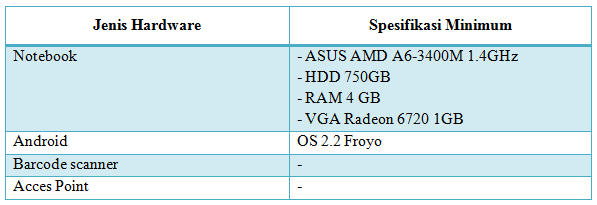
\includegraphics{gambar/hardware}
    \label{hardware}
\end{figure}

\section{Kebutuhan Perangkat Lunak}
Spesifikasi perangkat lunak yang digunakan untuk membangun aplikasi ini adalah : 

\begin{center}
Tabel 3.2. Kebutuhan Perangkat Lunak
\end{center}
\vspace{-0.5cm}
\begin{figure}[ht!]
  \centering
    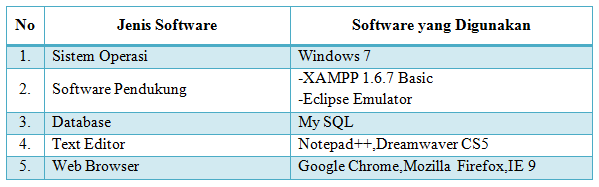
\includegraphics{gambar/software}
    \label{software}
\end{figure}

\section{Jadwal Kegiatan}
Penelitian direncanakan akan dilaksanakan selama tujuh bulan. Rincian rencana jadwal penelitian dicantumkan dalam tabel berikut :

\begin{center}
Tabel 3.3. Jadwal Penelitian
\end{center}
\vspace{-0.5cm}
\begin{figure}[ht!]
  \centering
    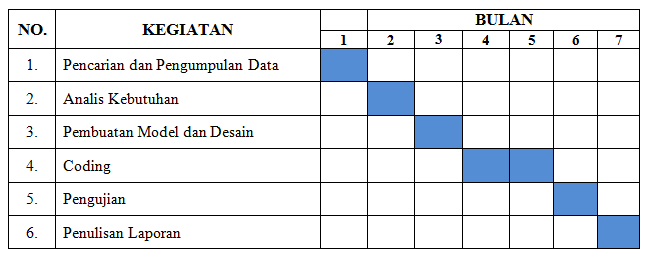
\includegraphics{gambar/jadwal}
    \label{jadwal}
\end{figure}


\begin{thebibliography}{9}

\bibitem[satu(2014)]{satu01}
Arinitweety. (2010, january 1). Voli Economici Venezia. Retrieved April 23, 2012, from Web Komunitas Event Organiser: http://eocommunnity.blogs.ukrida.ac.id/blogs/definisi-event-organizer/

\bibitem[dua(2014)]{dua02}
Isak, R. (2005). Dasar Pemrograman Berorientasi Objek dengan Java 2 (JDK 1.4). Yogyakarta: ANDI.

\bibitem[tiga(2014)]{tiga03}
Nazruddin Safaat, H. (2011). Pemrogaman Aplikasi Mobile Smartphone dan Tablet PC Berbasis Android. Bandung: Informatika.

\bibitem[empat(2014)]{empat04}
Surodjo, A. (2008). Definisi dan Sejarah Barcode.

\end{thebibliography}
\addcontentsline{toc}{chapter}{DAFTAR PUSTAKA}

\end{document}